\begin{figure}[htbp]
    \captionsetup[subfigure]{justification=centering}
    \centering
    \begin{subfigure}[b]{0.25\textwidth} % Decreased width to add space
        \centering
        
\includegraphics[width=\textwidth]{figures/featurelayersviz/low_channel.png}
        \caption{Lower Level Features}
    \end{subfigure}
    \hspace{0.05\textwidth} % Add space between subfigures
    \begin{subfigure}[b]{0.25\textwidth} % Decreased width to add space
        \centering
        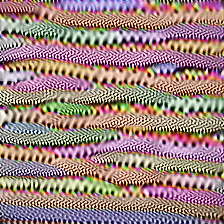
\includegraphics[width=\textwidth]{figures/featurelayersviz/medium_channel.png}
        \caption{Mid Level Features}
    \end{subfigure}
    \hspace{0.05\textwidth} % Add space between subfigures
    \begin{subfigure}[b]{0.25\textwidth} % Decreased width to add space
        \centering
        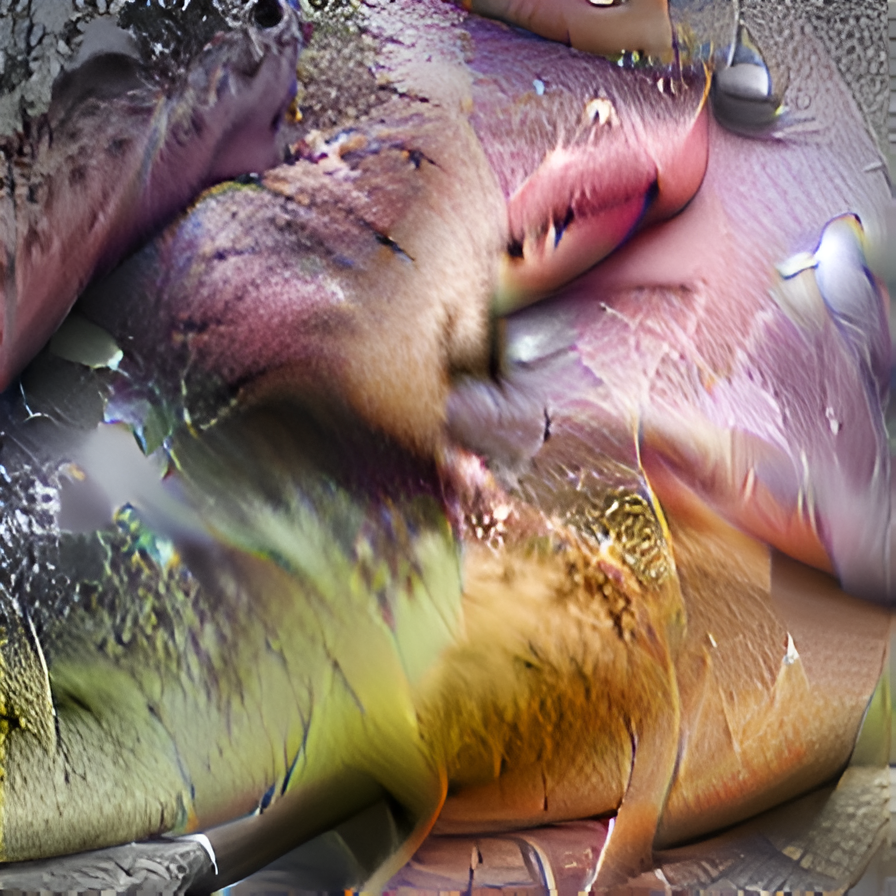
\includegraphics[width=\textwidth]{figures/featurelayersviz/late_channel.png}
        \caption{Higher Level Features}
    \end{subfigure}
    \caption{Illustration of Feature Representations at Different Levels}
    \label{fig:featurelayers}
\end{figure}